\documentclass[12pt]{article}
\usepackage[utf8]{inputenc}
\usepackage[left=2.5cm, right=2.5cm, top=2.0cm]{geometry}
\usepackage{sectsty}
\usepackage{graphicx}
\usepackage{amsmath}
\usepackage{amssymb}
% \usepackage{undertilde}
% \usepackage{kbordermatrix}
\usepackage{listings}
\usepackage{ulem}
\usepackage{soul}
% \usepackage{tikz}
% \usepackage{pgfplots}
% \pgfplotsset{compat=1.16}
\usepackage{siunitx}
\usepackage{pythonhighlight}
\usepackage{caption}
\usepackage{float}
\usepackage{url}
\usepackage{enumitem}
\usepackage{bm}
\usepackage{empheq}
\usepackage{tcolorbox}
\usepackage{framed}
\usepackage{xparse}
\usepackage{algorithm, algorithmic}
% \usepackage{algorithmic}
\usepackage{booktabs}
\usepackage{tabularx}
% ref packages
\usepackage{nameref}
% folowing  must be in this order
\usepackage{varioref}
\usepackage{hyperref}
\usepackage{cleveref}
\usepackage{mathtools}
\usepackage{longtable}
\DeclareMathOperator*{\argmax}{arg\,max}
% \usepackage[shortlabels]{enumitem}
\tcbuselibrary{breakable}
\allowdisplaybreaks


%  ---------------------- COMMANDS ---------------------------
% Double underline
\def\dunderline#1{\underline{\underline{#1}}}

% Shorten nonumber command
\def\nnb{\nonumber}

% Shorten boldsymbol command
\def\bs#1{\boldsymbol{#1}}

% Algorithmic newline
\def\algonewline{\STATE{ }}

% Eigenvectors of
\def\eigvecof{\text{eigenvectors of }}

% Eigenvalues of 
\def\eigvalof{\text{eigenvalues of }}

% Enclose in square brackets
\newcommand{\enclb}[1]{\left[#1\right]}
% Enclose in parenthesis
\newcommand{\enclp}[1]{\left(#1\right)}
% Enclose in curly brackets
\newcommand{\enclc}[1]{\left\{#1\right\}}

% Annotate first argument, text in second argument
\newcommand{\overtext}[2]{\overbrace{#1}^{\mathclap{\text{#2}}}}
\newcommand{\undertext}[2]{\underbrace{#1}_{\mathclap{\text{#2}}}}

% Normalization constant in multivariate normal
\newcommand{\mvnconst}[1]{\frac{1}{(2\pi)^{d/2} |#1|^{1/2}}}

% Exponential factor in multivariate normal
\newcommand{\mvnexpo}[3][x]{\exp \left[  -{\frac{1}{2}} (#1 - #2)^T #3^{-1} (#1 - #2) \right]}

% Multivariate normal
\newcommand{\mvn}[3][x]{\mvnconst{#3} \mvnexpo[#1]{#2}{#3}}

% For numbering in align* environment
\newcommand{\numberthis}{\addtocounter{equation}{1}\tag{\theequation}}

%  Sum notation w/ limits as argument and index as option
\newcommand{\sumlim}[3][i]{\sum\limits_{#1=#2}^{#3}}

%  Product notation w/ limits as argument and index as option
\newcommand{\prodlim}[3][i]{\prod\limits_{#1=#2}^{#3}}

%  Sum notation with only information beneath
\newcommand{\sumnolim}[1]{\sum\limits_{#1}}

%  Integral notation w/ limits as argument and index as option
\newcommand{\intlim}[2]{\int\limits_{#1}^{#2}}

%  Integral over whole domain notation, no args
\newcommand{\intinf}{\int\limits_{-\infty}^{\infty}}

%  Partial derivative notation, arg1: numerator, arg2: denominator
\newcommand{\pfrac}[3][ ]{\frac{\partial^{#1} #2}{\partial #3^{#1}}}

%  Derivative notation, arg1: numerator, arg2: denominator
\newcommand{\dvfrac}[3][ ]{\frac{\text{d}^{#1} #2}{\text{d} #3^{#1}}}

% When doing Gauss-Jordan, create arrow showing operations
\newcommand{\ro}[1]{\xrightarrow{\mathmakebox[\rowidth]{#1}}}

% ----------------------INVIRONMENTS---------------------------
% Item list with title
\newenvironment{titlemize}[1]{%
  \paragraph{#1}
  \begin{itemize}}
  {\end{itemize}}

  % Enum list with title
\newenvironment{titleenum}[1]{%
  \paragraph{#1}
  \begin{enumerate}}
  {\end{enumerate}}

  % Augmented matrix (matrix with vertical line)
\newenvironment{sysmatrix}[1]
  {\left(\begin{array}{@{}#1@{}}}
  {\end{array}\right)}

 % Make matrices with more spacing
\makeatletter
\renewcommand*\env@matrix[1][\arraystretch]{%
  \edef\arraystretch{#1}%
  \hskip -\arraycolsep
  \let\@ifnextchar\new@ifnextchar
  \array{*\c@MaxMatrixCols c}}
\makeatother

% \renewcommand*{\arraystretch}{1.5}

\newlength{\rowidth}% row operation width
\AtBeginDocument{\setlength{\rowidth}{3em}}

\floatname{algorithm}{Algorithm}
\renewcommand{\algorithmicrequire}{\textbf{Input:}}
\renewcommand{\algorithmicensure}{\textbf{Output:}}

\begin{document}
\title{\textbf{INF367A Project 2}}
\author{Naphat Amundsen}
\maketitle
\sectionfont{\fontsize{14}{15}\selectfont}
\subsectionfont{\fontsize{12}{15}\selectfont}
\subsubsectionfont{\fontsize{12}{15}\selectfont}
\graphicspath{ {./images/} }

\ifx
\begin{figure}[H]
	\centering
	\includegraphics[scale=0.8]{Figure_2}
	\caption{Insert caption here}
\end{figure}
\fi

\newcommand{\opGamma}{\operatorname{Gamma}}
\newcommand{\Um}{\underset{n \times k}{U}}
\newcommand{\Vm}{\underset{k \times m}{V}}
\newcommand{\Xm}{\underset{n \times m}{X}}
\newcommand{\neff}{N_{\text{eff}}}
\newcommand{\rhat}{\hat{R}}

\section*{Introduction}
    This project is about creating a bayesian recommender engine specifically for movie ratings. There are different types of recommender systems. For this project, we will focus on \textit{collaborative filtering} where we try to predict user preferences based on preferences. We are given the MovieLens 100K dataset, which essentially consists of movies, users and the users ratings for the movies. The dataset contains $100 000$ ratings from $943$ users on $1682$ movies. The data is sparse, because not every user has rated every movie. The task is to predict the users ratings on movies that they have not seen. 

    The recommender system is based on Bayesian matrix factorization, that is, we want to predict ratings as well as estimating the uncertainty in the predictions. We try using three different models to estimate the matrix factors.

\section{The models}
    The user-rating pairs can be represented with the matrix $\Xm$, where each row represents a user, and each column represents as movie. To predict the users' rating on unreviewed movies, we try to factorize matrix into two matrices $\Um, \Vm$ such that $UV \approx X$, where $k$ denotes the number of the latent dimensions of the factors. The matrices $U,V$ will be approximated using using Hamitonian Monte Carlo implemented in Stan \cite{HMC}.

    \subsection*{Data standard deviation}
        All the models share the same distribution for the data, that is $X_{ij}\sim N((UV)_{ij}, \beta)$. The prior for $\beta$ is chosen to be a gamma distribution with scale$=1$, and shape$=1$, which seems reasonable as we expect the data points to be close to whatever $UV$ estimates. Note that this is effectively an exponential distribution with rate $1$.
    
        \begin{figure}[H]
            \centering
            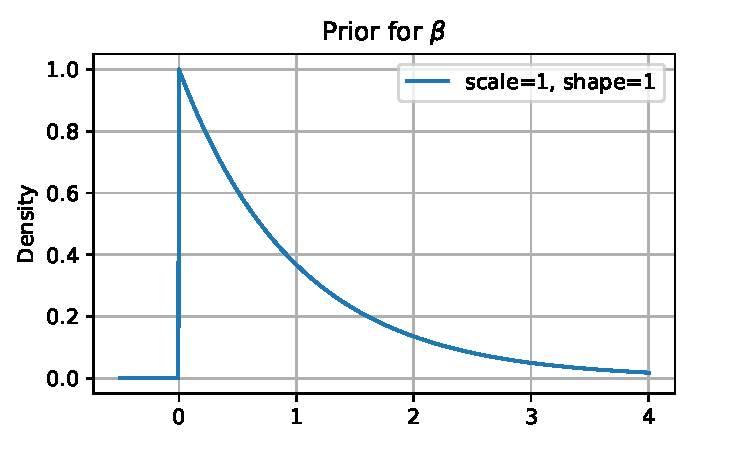
\includegraphics[width=0.5\textwidth]{betaprior.pdf}
            \caption{Probability density function for $\beta$, the assumed standard deviation of the data from the estimated values from $UV$.}
        \end{figure}
    
    \subsection{Normal model}
    This model is inspired from the "regular" way of doing Bayesian linear regression, that is the elements of $U$ and $V$ are normally distributed. To give more flexibility to the user, the normal distributions for $U$ and $V$ each has different sets of user specified parameters, that is the means and standard deviations. The data points are then assumed to be normally distributed, where the mean is what $UV$ is at the corresponding element, and the standard deviation assumed to be distributed by a gamma distribution with user specified values for shape and scale. The model rather is "vanilla", and will serve as a baseline to be beaten. We would say that it is reasonable to expect the model to at least be better than random.
    \begin{align*}
        U_{ij}  &\sim N(\mu_U, \sigma_U) \\
        V_{ij}  &\sim N(\mu_V, \sigma_V) \\
        \beta  &\sim \opGamma(a_\beta, b_\beta) \\
        X_{ij} &\sim N((UV)_{ij}, \beta) 
    \end{align*}

    User defined parameters: $\mu_U, \sigma_U, \mu_V, \sigma_V, a_\beta, b_\beta$.
    
    \vspace{3mm}
    We set the the means for the elements in $U$ and $V$ to be $0$, and set the standard deviations to be $5$, just to cover the range of the ratings within one standard deviation. That is: $\mu_U=0,\ \sigma_U=5,\ \mu_V=0,\ \sigma_V=5,\ a_\beta=1,\ b_\beta=1$.

    \subsection{Non-negative factorization model}
    The idea here is to constrain $U$ and $V$ to consist only of positive numbers, as the ratings are only positive after all. This model is very much like the normal model mentioned above, but the elements of $U$ and $V$ are gamma distributed instead.
    \begin{align*}
        U_{ij} &\sim \opGamma(a_U, b_U) \\
        V_{ij} &\sim \opGamma(a_V, b_V) \\
        \beta  &\sim \opGamma(a_\beta, b_\beta) \\
        X_{ij} &\sim N((UV)_{ij}, \beta) 
    \end{align*}

    User defined variables: $a_U, b_U, a_V, b_V, a_\beta, b_\beta$.
    
    \vspace{3mm}
    We specify the scale and shape such that the density "huddles" around $1$, as multiplying $\Um$ and $\Vm$ will involve a lot of multiplications and additions when reconstructing $\Xm$, which will have the flexibility to cover the whole range og ratings even if the elements of $U$ and $V$ are around $1$, thus we find it reasonable to expect values to not be very large. We achieve such a gamma distribution by setting the scale to $2$ and the shape to $1$.
    \begin{figure}[H]
        \centering
        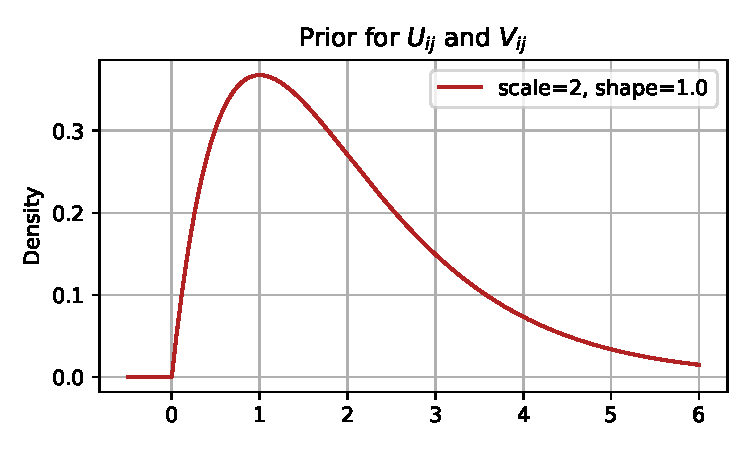
\includegraphics[width=0.5\textwidth]{nmfprior.pdf}
        \caption{Probability density function for the elements in $U$ and $V$.}
    \end{figure}
    To summarize: $a_U=2,\ b_U=1,\ a_V=2,\ b_V=1,\ a_\beta=1,\ b_\beta=1$.

    \subsection{ARD model}
    This model is inspired by the ARD (Automatic Relevance Determination) model used for regression tasks. This model can be viewed as an extension of the aforementioned "Normal model". The matrices $\Um$ and $\Vm$ are still assumed to be distributed with gaussians. However, the difference is that each column (essentially components) of $U$ and $V^T$ has their own standard deviations. The standard deviations are assumed to be distributed from a gamma distribution with user specified parameters. We denote the standard deviations for the columns with the array $\alpha$ of size $k$, where each element correspond to each column of $U$ and $V^T$.
    \begin{align*}
        \alpha_{j}  &\sim \opGamma(a_\alpha, b_\alpha) \\
        U_{ij}  &\sim N(\mu_U, \alpha_j) \\
        V^T_{ij}  &\sim N(\mu_V, \alpha_j) \\
        \beta  &\sim \opGamma(a_\beta, b_\beta) \\
        X_{ij} &\sim N((UV)_{ij}, \beta)
    \end{align*}

    User defined variables: $\mu_U, \mu_V, a_\alpha, b_\alpha, a_\beta, b_\beta$.
    
    \vspace{3mm}
    We specify the same parameters as the Normal model for the ARD model where we can, that is the means and standard deviations for $U$ and $V$. We are unsure how the $\alpha$ values for the ARD should take, so we pick parameters for the prior distribution that does such that it does not assume much. 
    \begin{figure}[H]
        \centering
        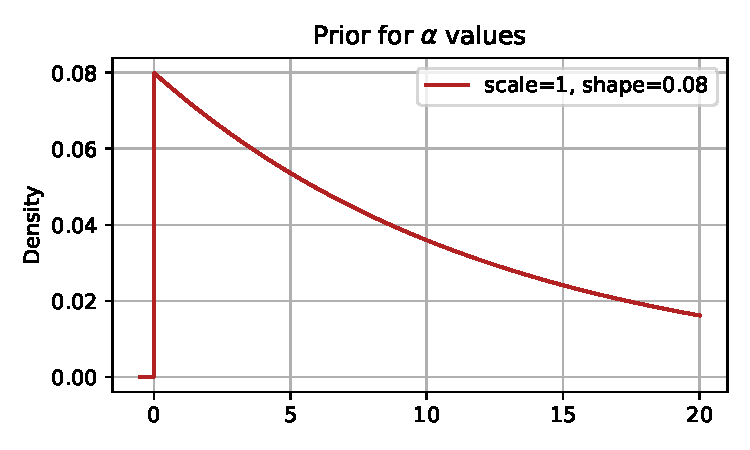
\includegraphics[width=0.5\textwidth]{alphaprior.pdf}
        \caption{Probability density for $\alpha$ values. Again, this is effectively equivalent to an expononential distribution. Note that the rate is quite low (compared to the one used for $\beta$).}
    \end{figure}
    To summarize the parameters for the ARD priors: $\mu_U=0,\ \sigma_U=5,\ \mu_V=0,\ \sigma_V=5,\ a_\alpha=1,\ b_\alpha=0.08, \ a_\beta=1,\ b_\beta=1$.

\section{Model selection}
We do model selection to find the best performing model on the dataset. There are many hyperparameters that can be tuned such as the scale and shape of gamma distributions for the $\beta$-value for the models. However, as the training time takes quite a while for each model, we limit the hyperparameter search to just finding a good value for $k$, that is the latent dimension of the matrix factors $\Um, \Vm$. We will subsample the data for the model selection part to speed up the process.

After determining the best candidate model the model selection, said candidate will be trained on $90\%$ of all the data, and then validated on the remaining $10\%$.

    \subsection*{Quick look at the data}
    A rating is an integer ranging from $1$ to $5$. As mentioned earlier, the dataset contains $100 000$ ratings from $943$ users on $1682$. That means we have a $943 \times 1682$ matrix, where only $100000$ elements are observed, implying we have a sparse matrix, where only $6.3\%$ of the elements are observed.  
    \begin{figure}[H]
        \centering
        \caption{Distribution of ratings.}
        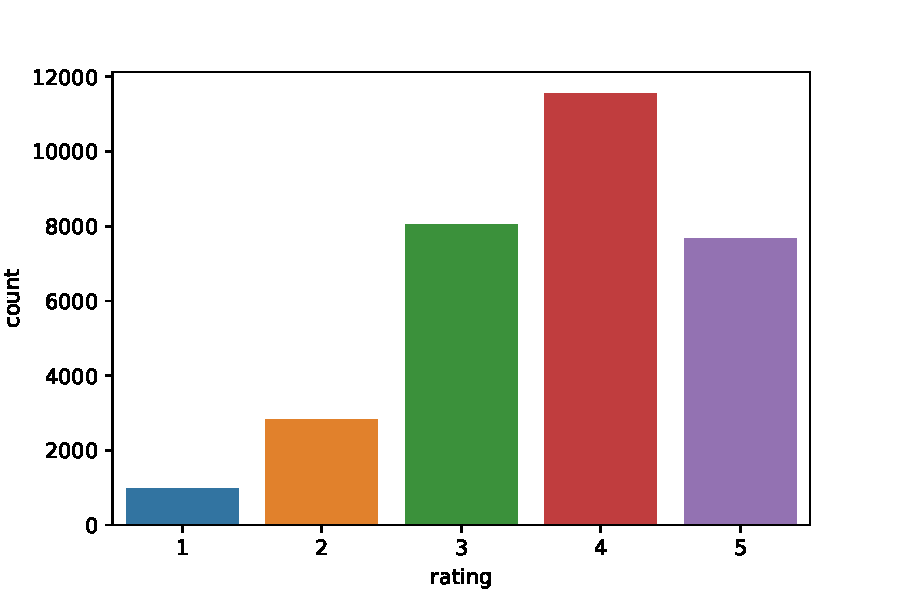
\includegraphics[width=0.6\textwidth]{ratings.pdf}
    \end{figure}
    Not only is the matrix rather sparse, but the ratings are also unbalanced, meaning we have an unbalanced dataset. This may lead to models that overfit to the most frequent ratings, that is the rating of $4$.  

    \subsection{Data subsampling}
    To speed up the model selection process we do model selection on a subset of the data. We subsample 250 users and 250 movies. The matrix is sparse, so we want to subsample the data such that we get the "dense parts" of the matrix. To do this we pick the top 250 users based on number of movies rated, then we pick the top 250 movies with the most ratings from said top users. This produces a $250 \times 250$ matrix with about $50\%$ observed elements. From the subset we create a train ($90\%$ of the subset) and a hold out set (the remaining $10\%$). The train set will be used for training, while the hold out set will be used for validation.

    \subsection{Model selection results}
    We try $1$ to $5$ latent dimensions for each model. We do $2000$ iterations using Stan's HMC sampler, and set the "max\_treedepth" control argument to $15$ (the warnings from Stan told to) when sampling for each model.

        \subsubsection*{Scoring metric}
        To score the models we take the mean absolute error of all the predicted ratings to the actual ratings. That is, for each sampled $U$ and $V$, we get a corresponding $\hat{X}$, which contains predictions for the movie ratings. We calcuate the absolute error of the ratings contained in $\hat{X}$ to the ratings in the validation set. We do this for every sampled pairs of $U$ and $V$, and then we calculate the mean of all the errors. 

    \begin{table}[H]
        \centering
        \caption{k is the latent dimension, train time shows training time in seconds, train MAE is the mean absolute error on the training set, while val MAE is the mean absolute error on the validation set. The table is sorted with respect to val MAE in ascending order (lower is better).}
        \label{table:modelselection}
        \begin{tabular}{llrr|rr}
            \toprule
            {} &         model &  k &  train time (seconds) &  train MAE &  val MAE \\
            \midrule
            1  &           ARD &  3 &             4748.8171 &     0.6510 &   0.6822 \\
            2  &  Non-negative &  3 &             2111.0567 &     0.6499 &   0.6827 \\
            3  &        Normal &  3 &             3204.8550 &     0.6488 &   0.6827 \\
            4  &           ARD &  4 &             5602.4438 &     0.6415 &   0.6832 \\
            5  &  Non-negative &  2 &             2071.6710 &     0.6630 &   0.6843 \\
            6  &           ARD &  2 &             4142.7847 &     0.6635 &   0.6845 \\
            7  &        Normal &  2 &             1749.6510 &     0.6628 &   0.6850 \\
            8  &  Non-negative &  4 &             2727.4210 &     0.6406 &   0.6860 \\
            9  &           ARD &  5 &             5765.4504 &     0.6327 &   0.6876 \\
            10 &        Normal &  4 &             3805.0494 &     0.6384 &   0.6900 \\
            11 &  Non-negative &  5 &             2528.1382 &     0.6321 &   0.6938 \\
            12 &        Normal &  5 &             5514.9162 &     0.6283 &   0.6997 \\
            13 &        Normal &  1 &             1099.4541 &     0.6991 &   0.7083 \\
            14 &  Non-negative &  1 &             1589.8258 &     0.6992 &   0.7084 \\
            15 &           ARD &  1 &             2599.5240 &     0.6992 &   0.7084 \\
            \bottomrule
        \end{tabular}
    \end{table}
    
    \begin{table}[H]
        \centering
        \caption{This table shows the min, max, mean and standard deviation of the $\bs{\rhat}$ values from the sampling of all the models. The order of the rows correspond to Table \ref{table:modelselection}. Rhat gives an indication of whether the model parameters have converged \cite{Rhat}. It should be noted that convergence does not imply that the sampling process managed to sample from the true posterior distribution. According to the Stan warnings, a $\rhat$ value for a parameter between 0.9 and 1.1 indicates likely convergence. Ideally, the $\rhat$ values should be $1$.}
        \label{table:rhats}
        \begin{tabular}{llr|rr|rr}
            \toprule
            {} &         model &  k &  Rhat min &  Rhat max &  Rhat mean &  Rhat std \\
            \midrule
            1  &           ARD &  3 &    0.9990 &    1.3138 &     1.0411 &    0.0887 \\
            2  &  Non-negative &  3 &    0.9990 &    1.0338 &     1.0032 &    0.0055 \\
            3  &        Normal &  3 &    0.9990 &    2.1189 &     1.2102 &    0.2135 \\
            4  &           ARD &  4 &    0.9990 &    1.3835 &     1.0594 &    0.0971 \\
            5  &  Non-negative &  2 &    0.9990 &    1.0250 &     1.0026 &    0.0044 \\
            6  &           ARD &  2 &    0.9990 &    1.2645 &     1.0478 &    0.0788 \\
            7  &        Normal &  2 &    0.9990 &    1.3543 &     1.0640 &    0.0827 \\
            8  &  Non-negative &  4 &    0.9990 &    1.0730 &     1.0052 &    0.0092 \\
            9  &           ARD &  5 &    0.9990 &    2.2013 &     1.1479 &    0.2843 \\
            10 &        Normal &  4 &    0.9990 &    2.4649 &     1.3759 &    0.3153 \\
            11 &  Non-negative &  5 &    0.9990 &    1.1202 &     1.0072 &    0.0126 \\
            12 &        Normal &  5 &    0.9990 &    1.9551 &     1.2106 &    0.2251 \\
            13 &        Normal &  1 &    0.9994 &    1.1562 &     1.0909 &    0.0238 \\
            14 &  Non-negative &  1 &    0.9991 &    1.2715 &     1.1814 &    0.0382 \\
            15 &           ARD &  1 &    1.0024 &    1.5671 &     1.2801 &    0.1115 \\
            \bottomrule
        \end{tabular}
    \end{table}

    \begin{table}[H]
        \centering
        \caption{This table shows the min, max, mean and standar deviation of the $\bs{\neff}$ (number of effective samples) values from the sampling. The order of the rows correspond to Table \ref{table:modelselection}. Number of effective samples is a estimate on how many samples of each model parameter got sampled from the true posterior \cite{Neff}.}
        \label{table:neffs}
        \begin{tabular}{llr|rr|rr}
            \toprule
            {} &         model &  k &  $\neff$ min &  $\neff$ max &  $\neff$ mean &  $\neff$ std \\
            \midrule
            1  &           ARD &  3 &    4.8574 & 1127.6726 &   275.7620 &  231.6963 \\
            2  &  Non-negative &  3 &   40.4421 & 1677.8139 &   318.3954 &  223.1981 \\
            3  &        Normal &  3 &    3.4360 & 1020.3357 &    10.5009 &   28.1623 \\
            4  &           ARD &  4 &    4.8997 & 1571.0058 &   220.2744 &  272.0015 \\
            5  &  Non-negative &  2 &   33.8124 & 1403.8710 &   234.1758 &  191.7673 \\
            6  &           ARD &  2 &    5.5987 & 1657.3678 &   297.9770 &  320.3376 \\
            7  &        Normal &  2 &    3.9082 & 1127.2144 &    10.0871 &   37.3944 \\
            8  &  Non-negative &  4 &   16.0936 & 1799.1824 &   187.5072 &  157.2839 \\
            9  &           ARD &  5 &    2.9357 & 1231.9205 &   136.8569 &  228.5099 \\
            10 &        Normal &  4 &    2.7750 & 1068.2205 &     8.1337 &   25.1019 \\
            11 &  Non-negative &  5 &   35.9622 & 1523.1771 &   268.6275 &  162.7551 \\
            12 &        Normal &  5 &    3.3734 &  894.0220 &    10.0690 &   20.1732 \\
            13 &        Normal &  1 &   10.4850 & 1007.2907 &    21.6554 &   47.9306 \\
            14 &  Non-negative &  1 &    5.2699 &  771.6474 &    10.6626 &   38.0074 \\
            15 &           ARD &  1 &    4.3445 &  586.1205 &     8.2810 &   25.9324 \\
            \bottomrule
        \end{tabular}
    \end{table}

    It clearly seems to be that $3$ latent dimensions, that is the $k$ value for $\Um$ and $\Vm$, is the most optimal one with respect to validation MAE since the top three are all the three different types of models, all with $k=3$. The top 3 in ascending order is ARD, Non-negative and Normal, with the validation MAEs of $0.6822, 0.6827, 0.6827$ respectively. The scores are somewhat close to each other, but let us assess the convergence ($\rhat$) and the number of effective samples. 

    \vspace{3mm}
    We assess table \ref{table:rhats} and \ref{table:neffs} to get some indication on the convergence and $\neff$. The Non-negative model manages to get the best indications for convergence, the mean $\rhat$ is closest to one ($1.0032$), and has least variance ($0.005$) compared to the others. It also manages to get the highest value for mean number of effective samples ($318$), but with a rather high standard deviation of around $223$ (we want to have high mean and low standard deviation). The ARD model comes in second with the mean $\rhat$ of $1.04$ and mean $\neff$ of $275$. The Normal model looks rather horrible with bad convergence (mean $\rhat$ of $1.21$), and a very low mean $\neff$ of $10$, so we will not take it into any other further consideration. To get a closer look at the $\rhat$ and $\neff$ values for the ARD and the Non-negative model, we plot the correspoding histograms.

    \begin{figure}[H]
        \centering
        \caption{Here we see the $\rhat$ histograms on the left, and the $\neff$ histograms on the right. The top histograms shows the values from the ARD model, the middle histograms shows the values from Non-negative model, whilst the bottom histograms shows the top two histograms together.}
        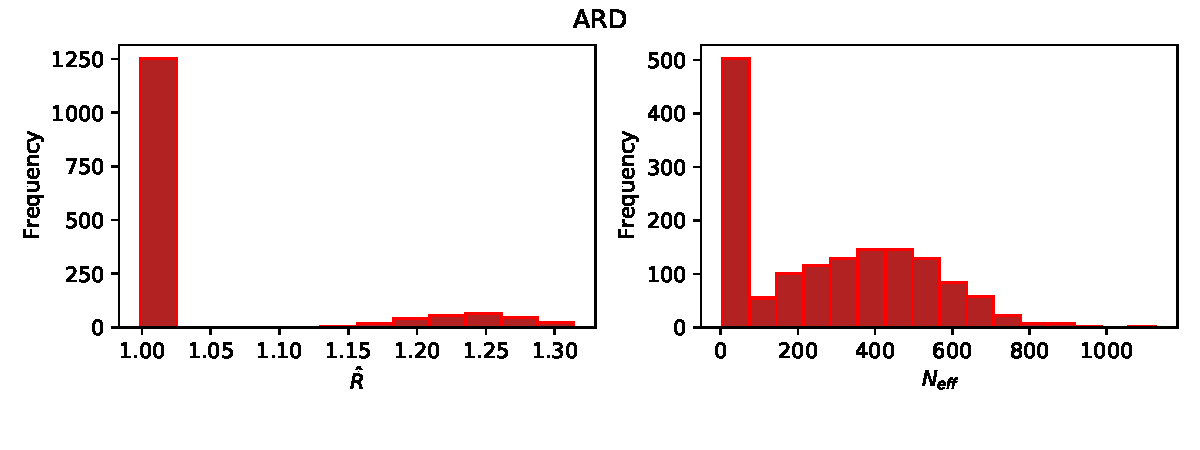
\includegraphics[width=0.85\textwidth]{ARD_hists.pdf}
        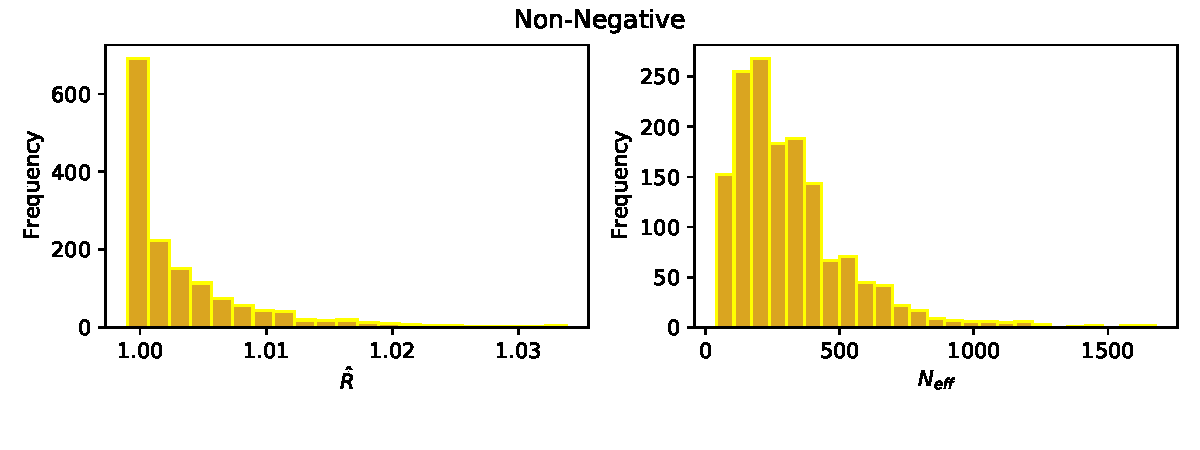
\includegraphics[width=0.85\textwidth]{NMF_hists.pdf}
        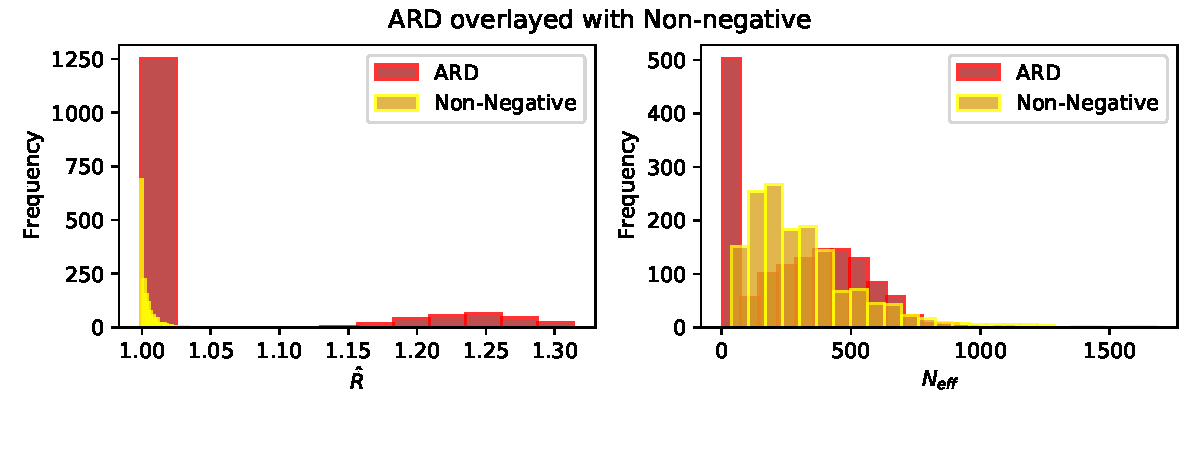
\includegraphics[width=0.85\textwidth]{ARDNMF_hists.pdf}
    \end{figure}

    We can see that the Non-negative model fares much better regarding the $\rhat$ values, the $\rhat$ values for the parameters are clearly much closer to $1$ overall compared to ARD. Regarding the number of effective samples we see that the Non-negative model "looks better", as it does not have that extreme peak at the low number bin for $\neff$ opposed to the ARD model. However, if one ignores the peak on the $\neff$ histogram for the ARD model, it seems to be that the ARD manages to get more effective samples for the parameters that "makes it". 

    We conclude that the Non-negative model is the overall winner of the model selection, even if it got second place regarding the MAE on the validation set, but has way better indication of convergence opposed to ARD, and has a much nicer looking histogram of $\neff$, which indicates that it probably managed to sample more from the true posterior. This decision is more of a Bayesian way of thinking. 

\section{Evaluating the best model}
We train the best candidate from the model selection, that is the Non-negative model using $3$ latent dimentions on a much larger amount of data. It should be noted that we effectively scrambled the data quite a bit during the early stages of experementing (we didn't seed in the beginning), thus we don't really have a proper test set, that is data that we have not touched whatsoever.

\vspace{5mm}
Using the whole dataset of $100000$ ratings, we create yet another train and validation set, where $90\%$ is used for the training set, and the rest for validation.

\begin{figure}[H]
    \centering
    \caption{We visualize the credible intervals for the validation ratings. Each spaghetti colored vertical line represents the $95\%$ credible interval of a rating from the predictive distribution. Each credible interval is computed from $400$ samples from the predictive distribution. The spaghetti sauce colored dots are the means of predictive samples. The yellow dots are the true ratings.}
    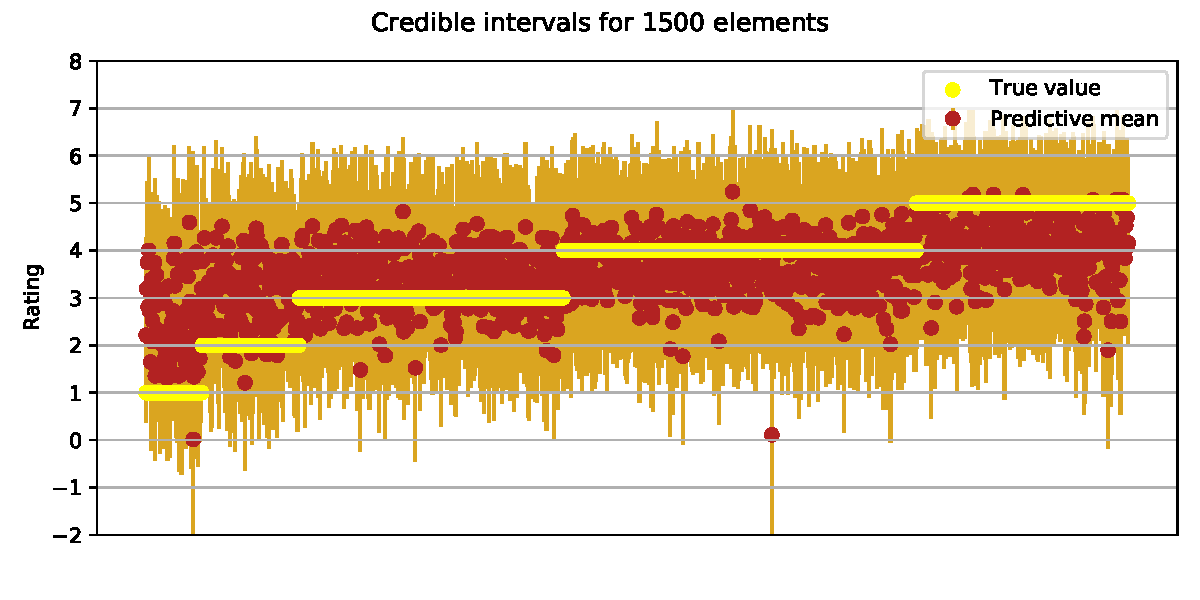
\includegraphics[width=\textwidth]{credibles.pdf}
\end{figure}
It does not look that great, at least we have some kind of trend, but the model does not have much credibility as the credible intervals are humongous. 

\section{Discussion}
    \subsection*{Bad Rhat and low effictive samples}
    Some models had low convergence, while some had low effective samples, and some were low on both. As an attempt to mitigate said problems, we simply tried to increase the number of sampling iterations. We ended up using 2000 iterations for both the model selection and model evaluation. We did not see that much of a difference between 1200 sampling iterations and 2000 when it came convergence, but of course we could generally expect a little higher number of effective samples at the cost of computating times.

    \subsection*{Extremely sampling time when many datapoints for Non-negative model}
    For some reason, training the Non-negative model on $900000$ ratings was extremely slow (2000 iterations, max\_treedepth=15). It took $144172$ seconds to finish, that is a bit over $40$ hours! 

% \bibliographystyle{apalike}
\bibliographystyle{ieeetr}
\bibliography{citations}

\end{document}
